\chapteropen
\chapter{Discussion and Implications}
\label{ch:discussion}
\hypertarget{ch:discussion}{}
\glsresetall
\quoteFive

\section{Overview: Compact Stellar Systems as Environmental Tracers}

In the preceding chapters, we have used \glspl{css} to investigate the effects of environmental processing in the dense core of the Coma Cluster. We focus on \glspl{css} in general, and \glspl{gc} in particular, because they are long-lived dynamical tracers of the processes experienced by their host galaxies \citep[\eg][]{Forbes_2018a, Beasley_2020}. In the central $\sim\qty{1}{\mega\parsec}$ of the Coma Cluster, this makes them especially useful probes of how dense environments reshape galaxy halos and their surrounding stellar systems. Across the thesis, we have built a picture of the spatial distribution, luminosity function, and color structure of \glspl{gc} and \glspl{ucd} throughout the cluster core. Taken together, these results indicate that stripping, redistribution, and mixing of \glspl{gc} are active in the Coma core. However, they also show that the observable signatures of this processing depend strongly on local \gls{gcs} structure, galaxy properties, and the \gls{gc} subpopulation under consideration.

\begin{sidewaysfigure}
    \centering
    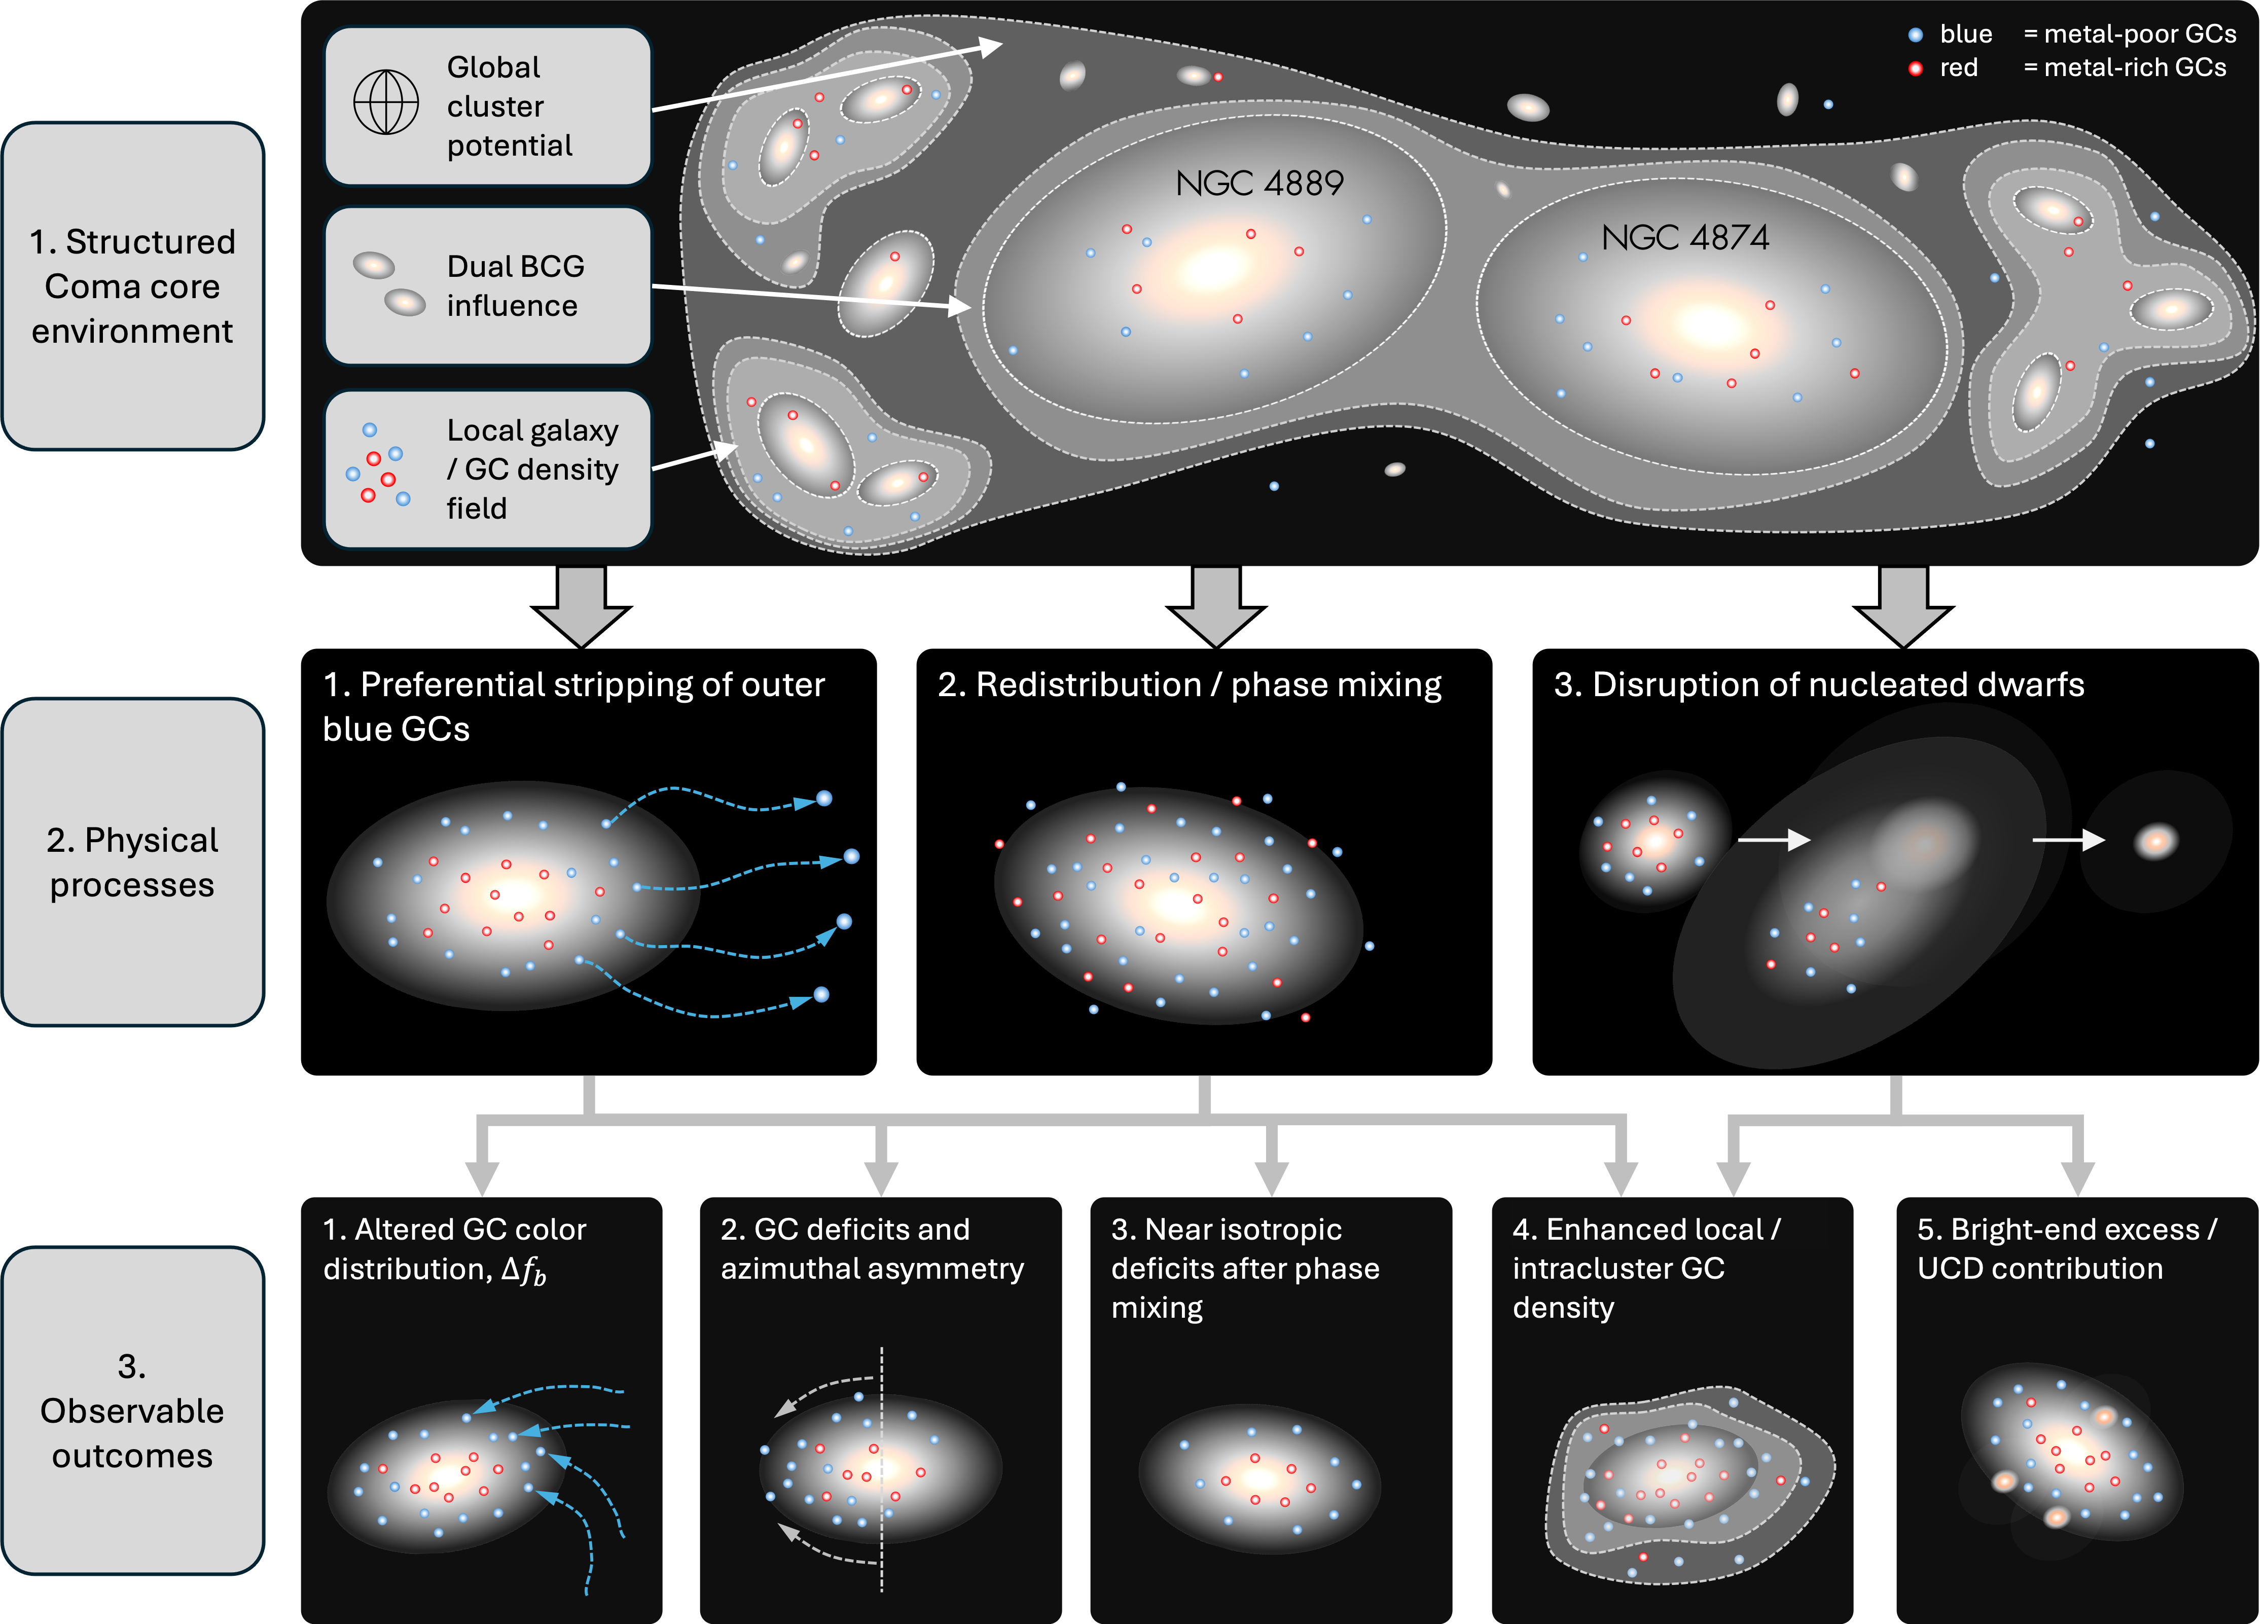
\includegraphics[width=0.95\textheight]{figures/discussion/Schematic.png}
    \caption[Schematic interpretation of environmental processing in the Coma Cluster core.]{
    Schematic interpretation of environmental processing in the Coma Cluster core. 
    The figure summarizes how the global cluster potential, dual \gls{bcg} environment, and local overdensities may preferentially strip and redistribute extended blue \glspl{gc}, producing altered metallicity mixes, deficient or asymmetric \glspl{gcs}, enhanced intracluster \gls{gc} density, and a possible contribution to the bright end of the \gls{css} population. 
    (Credit: Author)
    }   
    \label{fig:schematic}
\end{sidewaysfigure}

To guide the discussion, we refer to \cref{fig:schematic}, which summarizes the working physical picture that has emerged from the analyses presented in this thesis. The schematic is not intended to represent a single evolutionary pathway, nor a universal sequence of processing steps experienced by every cluster galaxy. Instead, it outlines a set of linked processes through which the dense cluster environment can imprint itself on \gls{css} populations. In this picture, the Coma core acts as a structured tidal field shaped by the global cluster potential, the influence of the dual \glspl{bcg}, and local galaxy and \gls{gc} overdensities. The most weakly bound components of a galaxy's \gls{gcs}, especially the more spatially extended blue \gls{gc} population, are preferentially stripped and redistributed. This can produce altered metallicity mixes relative to the cluster mean, deficient or asymmetric \glspl{gcs}, enhanced local or intracluster \gls{gc} densities, and a contribution from stripped nuclei to the bright end of the \gls{css} population. 

The following sections first discuss the evidence that the Coma core contains a structured population of redistributed \glspl{css}. We then consider how \gls{gc} deficits, asymmetries, and color-subpopulation trends constrain the mechanisms responsible, before placing these results in the broader context of galaxy evolution in dense environments.

% --------------------------------------
% New section - discussing the structure of the environment in the Coma Cluster, specifically the multi-scale structure, including influences from local, BCG and global potential of the cluster.
\section{Multi-scale Environmental Structure in the Coma Cluster}

\begin{claimquote}
The core of the Coma Cluster is not a smooth, radially symmetric environment; its \gls{css} population reflects a structured field shaped by the global cluster potential, the dual \glspl{bcg}, and local overdensities.
\end{claimquote}

Although the global cluster potential provides the large-scale gravitational field, the environmental signatures identified in this thesis are not governed by cluster-centric distance alone. Instead, as summarized in the upper part of \cref{fig:schematic}, the results point to a structured, multi-scale environment in which the dual \glspl{bcg}, local galaxy overdensities, and the \gls{gc} density field all contribute to the tidal and dynamical conditions experienced by galaxies in the core. 

This interpretation follows most directly from Chapter~\ref{ch:chapter4}, where \Dfb\ shows only a weak correlation with cluster-centric radius. The weakness of this trend, and its sensitivity to the choice of physically motivated cluster center, indicate that projected radius alone cannot capture the environmental field experienced by galaxies in the Coma Cluster core. The same conclusion is supported by the spatial structure identified in Chapter~\ref{ch:chapter2}: the global \gls{ucd} distribution is highly non-uniform, with density enhancements around the dual \glspl{bcg} and other systems such as IC~4051, as well as apparent bridges and voids. Chapter~\ref{ch:paper-example} further reinforces this picture, showing that the \gls{gc} density field across the cluster core contains detailed structure associated with individual galaxies, including both local overdensities and apparent deficits.

Importantly, the weakness of the cluster-centric trends should not be interpreted simply as an absence of environmental information. Instead, the sensitivity of these trends to the adopted center may itself reflect the dynamical state of the core of the Coma Cluster. If the \gls{css} population were fully mixed with respect to a single, relaxed cluster potential, one might expect a more stable radial signal independent of the precise center definition. The fact that the radial trends vary when measured from the X-ray peak, \gls{sz} peak, geometric center, or dual-\gls{bcg} midpoint suggests that the \gls{gc} population still retains memory of Coma's anisotropic assembly history. This is consistent with a core shaped by the dual \glspl{bcg}, infalling substructure, and local tidal perturbations, rather than by a smooth radially isotropic potential.

This multi-scale view is also consistent with the broader picture of cluster cores as dynamically structured environments rather than relaxed, featureless potentials. For example, recent deep imaging of the \gls{icl} around the core of the Coma Cluster by \citet{Jimenez-Teja_2025} reinforces this picture, showing a heterogeneous and clumpy \gls{icl} distribution around NGC~4874 and NGC~4889, consistent with an unrelaxed core and ongoing group dissolution. On even larger scales, weak-lensing measurements by \citet{HyeongHan_2024} show that the Coma Cluster is connected to intracluster filaments aligned with the surrounding supercluster structure, emphasizing that the cluster core is embedded within an anisotropic assembly environment. 

The \gls{css} population itself also shows this structured environment. Previous studies, for example, \citet{Peng_2011, Madrid_2018} have identified a substantial \gls{icgc} population, including bridging between galaxies, as well as large-scale overdensities associated with NGC~4889, NGC~4874, and IC~4051. Recent X-ray studies likewise show that the Coma Cluster is dynamically disturbed; for example \citet{Churazov_2021} find that the NGC~4839 group (south-west of the cluster core) interacts with the main cluster and leaves behind an extended gaseous substructure or bridge. This distinction between global cluster-centric environment and local density is consistent with recent work \citep[\eg][]{deVos_2024} showing that galaxy evolution in clusters depends on a complex interplay between cluster-centric distance, local environment, and galaxy properties.

Physically, this means that galaxies in the Coma Cluster core are unlikely to experience a single, smoothly varying tidal field. Instead, their \glspl{gcs} are shaped by a combination of global cluster tides, local perturbations from nearby massive galaxies, high-speed encounters, and the time-dependent influence of the dual \glspl{bcg}. These processes need not act in the same direction or on the same timescale. The outer \gls{gc} halo of a galaxy may therefore be truncated, distorted, or partially stripped depending on its orbit, its passage relative to the \glspl{bcg}, and the local density of galaxies and intracluster material. This provides a natural explanation for why environmental signatures in this thesis are strongest in local or \gls{bcg}-related diagnostics, and weaker when measured only as a function of cluster-centric radius.

The structured nature of the environment is particularly important for \glspl{gc}, because different parts of a \gls{gcs} respond differently to tidal processing. The centrally concentrated red \gls{gc} population is expected to remain more closely bound to the stellar body of the host galaxy, while the more spatially extended blue population is more easily affected by external tides. A multi-scale tidal field can therefore alter not only the total number of \glspl{gc} associated with a galaxy, but also the relative balance of blue and red subpopulations. In this sense, the \gls{gc} density field is not simply a background component to be removed, but part of the physical record of stripping, redistribution, and mixing in the cluster core.

This interpretation does not imply that the global cluster potential is unimportant. Rather, it suggests that its effects are filtered through projection, orbital history, and local substructure. Because the present analysis is based on projected positions and photometric \gls{gc} samples, we cannot assign individual galaxies to unique dynamical histories, nor can we distinguish all cases of direct stripping from older, phase-mixed redistribution. Similarly, high local \gls{gc} density should not be interpreted as a causal agent by itself; it is more likely a tracer of regions where stripping, accretion, and intracluster mixing have already deposited \glspl{css}. The relevant conclusion is therefore not that cluster-centric radius has no physical meaning, but that it is insufficient on its own to explain our observations.

The broader consequence is that environmental processing in the Coma Cluster core should be treated as a multi-scale phenomenon. Cluster-centric radius, \gls{bcg} proximity, local \gls{gc} density, and galaxy-scale asymmetry do not necessarily identify the same systems because they are sensitive to different aspects of the cluster environment. This explains why the samples highlighted by different diagnostics in Chapter~\ref{ch:chapter4} overlap but are not identical. Rather than weakening the environmental interpretation, this heterogeneity is itself part of the signal: \glspl{css} preserve the imprint of a structured cluster core in which stripping and redistribution occur locally, anisotropically, and over a range of timescales.

% --------------------------------------
% New section - discussing the local GC density which arises from environmental processing, and remains as a fossil record of that processing.
\section{The Local GC Density Field as a Record of Environmental Processing}

\begin{claimquote}
The local \gls{gc} density field is not simply a background component, but a spatial record of accumulated stripping, redistribution, and mixing in the Coma Cluster core.
\end{claimquote}

Having established that the Coma Cluster core is not well described by a smooth, radially isotropic environment, the local \gls{gc} density field should not be treated only as a background component. In this thesis, local \gls{gc} density functions both as a source of contamination for galaxy-scale measurements and as a physical tracer of redistributed \glspl{css}. This dual role is central to interpreting the environmental trends identified in Chapter~\ref{ch:chapter4}. As shown schematically in \cref{fig:schematic}, the local \gls{gc} density field is part of the outcome of environmental processing: it marks regions where stripping, redistribution, and mixing have accumulated \gls{css} over time.

The strongest environmental correlations in Chapter~\ref{ch:chapter4} are associated with local \gls{gc} density and, to a lesser extent, \gls{bcg}-related metrics, rather than with projected cluster-centric radius alone. This suggests that the blue-fraction diagnostic is responding most clearly to the immediate compact-object environment around each galaxy. Similarly, the spatial density maps in Chapter~\ref{ch:paper-example} show that this local field contains both galaxy-associated structure, anisotropic overdensities and voids, as well as more diffuse features that plausibly trace intracluster or redistributed \glspl{gc}.

Previous foundational studies of \glspl{gc} in Coma \citep[\eg][]{Peng_2011, Madrid_2018} have identified a substantial \gls{icgc} population, including bridge-like structures between the central galaxies and large-scale overdensities associated with NGC~4889, NGC~4874, and IC~4051. More recently, \citet{Jimenez-Teja_2025} revealed a clumpy intracluster component around NGC~4874 and NGC~4889 through deep \gls{icl} imaging of the Coma core, which is consistent with the spatial complexity seen in the \gls{gc} field.

However, this interpretation is not unique to Coma. In Virgo, large-scale intracluster \gls{gc} substructures have been detected on scales larger than individual galaxy halos, with the blue \gls{gc} population especially extended and naturally interpreted in terms of stripping from cluster galaxies \citep{Lee_2010b}. Tidal-stripping studies of Virgo early-type galaxies likewise find that environmental effects are strongest for the blue \gls{gc} population, consistent with its more extended spatial distribution and greater susceptibility to the cluster potential and galaxy--galaxy interactions \citep{Coenda_2009}. More recently, Wide-field Euclid observations of the Perseus Cluster \citep{Kluge_2025} and Fornax cluster \citep{Saifollahi_2025} have shown that the \gls{icl} and \glspl{icgc} share a coherent spatial distribution over several hundred kiloparsecs, suggesting either a common origin or a common governing potential. 

Together, these studies support the interpretation of the local \gls{gc} density field as a physical imprint of stripping and redistribution, rather than as a purely statistical background. In this view, diffuse intracluster components such as the \gls{icl} and \glspl{icgc} are not only by-products of environmental processing, but also tracers of the cluster potential, accretion history, and cumulative assembly of the cluster core.

There are, however, important limits to this interpretation. The local \gls{gc} density field is a composite quantity, containing some combination of galaxy-associated \glspl{gc}, extended \gls{bcg} halos, \glspl{icgc}, stripped material, older phase-mixed debris, and residual contamination. A local overdensity should therefore not be interpreted as a single causal agent, nor as evidence for one specific stripping event. Instead, it is best understood as a projected tracer of the cumulative dynamical history of the region. In this sense, the same \gls{gc} field can be both an observational background for galaxy-scale measurements and a physical signal of environmental processing in the cluster core.

Thus, the local \gls{gc} density field should be regarded as a physically meaningful but non-unique record of environmental processing. It identifies regions where stripping, redistribution, and intracluster mixing have likely shaped the \gls{css} population, but it does not by itself isolate the mechanisms, progenitors, or timescales responsible. A complementary diagnostic is therefore needed: not only where \glspl{gc} are found in the cluster core, but which \gls{gc} subpopulations are most affected. This motivates the next section, where we consider the relative sensitivity of the blue \gls{gc} subpopulation to environmental processing.

% --------------------------------------
% New section - discussing blue globular clusters their preferential response due to their more extended spatial distribution thoughout the cluster
\section{The Preferential Response of the Blue Globular Cluster Population}

\begin{claimquote}
The extended blue \gls{gc} population provides the clearest signature of environmental processing because it is expected to be more weakly bound and more easily stripped than the centrally concentrated red population.
\end{claimquote}

The previous section argued that the local \gls{gc} density field provides a fossil record of environmental processing in the Coma Cluster core. However, this record is inherently ambiguous: it identifies regions where stripping, redistribution, and mixing have likely occurred, but it does not by itself determine the timing of those events or distinguish between the mechanisms responsible. To move beyond the density field alone, we therefore turn to variations in the metal-rich (red) and metal-poor (blue) \gls{gc} subpopulations. Across the analyses presented in this thesis, the blue \gls{gc} population emerges as the more sensitive tracer of environmental processing. In the framework of \cref{fig:schematic}, this corresponds to the preferential stripping of the extended blue-\gls{gc} component, whose larger spatial extent makes it more vulnerable to external tides than the centrally concentrated red population.

This conclusion is supported by two complementary results. In Chapter~\ref{ch:chapter1}, we showed that the spatial distribution of the blue \gls{ucd} subpopulation is more extended than that of the red \gls{ucd} subpopulation. Although the \gls{ucd} and \gls{gc} samples are not identical, this result is consistent with the broader picture that the blue, metal-poor \gls{css} component is more spatially extended and therefore more exposed to environmental processing. In Chapter~\ref{ch:chapter4}, we used the diagnostic \Dfb{}, which traces the blue \gls{gc} fraction excess relative to the cluster-wide mean, to test how the subpopulation mix varies with environment. In that analysis, environmental trends are most clearly expressed through changes in the blue \gls{gc} fraction. Because this diagnostic measures the relative balance of the metal-poor and metal-rich components, it does not by itself isolate changes in either subpopulation independently. However, when combined with the expected spatial vulnerability of blue \glspl{gc}, the result supports the interpretation that the metal-poor component is the more sensitive tracer of environmental processing.

This interpretation is physically motivated by the distinct spatial distributions of the two main \gls{gc} subpopulations. Blue, metal-poor \glspl{gc} are generally associated with the more extended halo component of a \gls{gcs}, while red, metal-rich \glspl{gc} are more centrally concentrated and more closely coupled to the stellar body of the host galaxy \citep[\eg][]{Brodie_2006, Harris_2010a, Forbes_2018a}. The extended spatial distribution of the blue population makes it more vulnerable to external tides, so environmental processing is expected to first affect the blue-dominated outskirts of galaxy \glspl{gcs}. This expectation is supported by studies of the Virgo Cluster, where environmental trends in \gls{gc} specific frequency are strongest for the blue population and have been interpreted as evidence for tidal stripping near the cluster center \citep{Coenda_2009}. Large-scale intracluster \gls{gc} structures in Virgo also show an especially extended blue component, consistent with metal-poor clusters being preferentially redistributed into the cluster environment \citep{Lee_2010b, Durrell_2014}. A recent paper by \citet{Reina-Campos_2026} similarly found that bright blue \glspl{gc} trace the cluster mass distribution more closely than red \glspl{gc}, consistent with their more spatially extended nature. This supports the view that blue \glspl{gc}, once redistributed beyond their original host halos, become sensitive tracers of the cluster-scale potential rather than only of individual galaxy halos.

In this context, changes in \Dfb\ are naturally interpreted as changes in the relative balance of the metal-poor and metal-rich \gls{gc} components. The use of this type of diagnostic builds on the established result that \gls{gc} color distributions encode systematic variations in subpopulation mix across early-type galaxies \citep{Peng_2006}. Variations in the relative numbers of blue and red \glspl{gc} are therefore physically meaningful, since \gls{gc} formation efficiencies and specific frequencies reflect both early star formation and subsequent assembly history \citep{Peng_2008}. The metal-poor \gls{gc} population has also been used explicitly as an environmental tracer in Virgo dwarfs, where comparisons of blue-\gls{gc} mass specific frequency were used to test cluster transformation scenarios \citep{Sanchez-Janssen_2012}. More recent studies of \gls{gcs} scaling relations likewise treat \gls{gc} richness and radial structure as quantities sensitive to satellite/central status and environmental processing \citep{DeBortoli_2022}.

The main caveat is that \Dfb\ is a relative diagnostic. It does not by itself distinguish whether blue clusters have been preferentially removed, red clusters have been comparatively preserved, or the surrounding intracluster population has altered the measured mixture. Nevertheless, when considered alongside the more extended spatial distribution of blue \glspl{gc}, the environmental modulation of \Dfb\ supports the interpretation that the metal-poor component is the clearest tracer of environmental processing in the Coma Cluster core. This diagnostic identifies the population most sensitive to environmental influence, but it does not directly encode the direction or timing of that processing. For that, we turn next to the azimuthal structure of \glspl{gcs} and the use of asymmetry as a diagnostic of stripping geometry and timescale.

\section{Asymmetry as a Diagnostic of Stripping Geometry and Timescale}

\begin{claimquote}
    The azimuthal structure of deficient \glspl{gcs} provides information about stripping geometry and relative timescale, with asymmetric systems likely preserving more recent or directional signatures.
\end{claimquote}

The previous section identified the blue \gls{gc} population as the component most sensitive to environmental processing. However, changes in the blue fraction alone do not determine the geometry or timing of that processing. A reduced or altered blue component may result from recent stripping, older phase-mixed redistribution, or a more symmetric truncation of the outer \gls{gcs}. In the framework of \cref{fig:schematic}, these possibilities correspond to different observable outcomes of the same broad environmental process. We therefore turn to the azimuthal structure of galaxy \glspl{gcs}: recently stripped or tidally disturbed systems may retain directional signatures, whereas older or more thoroughly mixed systems are expected to appear increasingly isotropic.

\begin{table}[ht]
\centering
\caption{Possible origins of deficient GCSs and their expected signatures.}
\label{tab:gcs_deficit_scenarios}
\scriptsize
\begin{adjustbox}{max width=\textwidth}
\begin{tabular}{p{0.20\textwidth}p{0.23\textwidth}p{0.26\textwidth}p{0.23\textwidth}}
\doubletoprule
Scenario & Expected \gls{gcs} signature & Possible environmental interpretation & Key ambiguity \\
\midrule
Intrinsic low \gls{gc} formation efficiency &
Low total \gls{gc} population, but not necessarily strong asymmetry or truncation &
The galaxy may have formed relatively few \glspl{gc} at early times, rather than losing them later &
Can mimic an environmentally stripped system if only total \gls{gc} counts are considered \\

Recent or ongoing directional stripping &
Deficient \gls{gcs} with azimuthal asymmetry, lopsided structure, or offsets relative to the galaxy &
Outer \glspl{gc}, especially blue \glspl{gc}, may be actively stripped by local tides, BCG influence, or galaxy--galaxy encounters &
Projection and incomplete spatial coverage can complicate the interpretation of asymmetry \\

Older stripping or pre-processing &
Low \gls{gc} counts with weak or no remaining azimuthal asymmetry &
The galaxy may have been stripped before entering the present Coma Cluster core, or during an earlier passage through the dense environment &
Phase mixing can erase directional signatures, making old stripping difficult to distinguish from intrinsic deficiency \\

Approximately symmetric tidal truncation &
Reduced outer \gls{gc} halo, potentially with little azimuthal structure &
A smooth component of the cluster or BCG tidal field may remove the weakly bound outskirts of the \gls{gcs} &
May resemble both intrinsic deficiency and old phase-mixed stripping \\

Local intracluster/background contamination &
Apparent changes in \gls{gc} counts, color mix, or density structure near the galaxy &
The surrounding \gls{icgc} population may trace previously stripped material in the local environment &
Difficult to separate galaxy-associated \glspl{gc} from intracluster or redistributed \glspl{gc} using photometry alone \\
\bottomrule
\end{tabular}
\end{adjustbox}
% \tablecomments{
% }
\end{table}
This interpretation is motivated by the diversity of \gls{gcs} structures identified in Chapter~\ref{ch:paper-example}. Among galaxies with deficient \gls{gc} populations, some systems show clear azimuthal asymmetry, while others are nearly isotropic despite having reduced \gls{gc} counts. This diversity suggests that \gls{gc} loss is not a single-stage process. A summary of the possible origins of \gls{gcs} deficits is given in \cref{tab:gcs_deficit_scenarios}. In this context, asymmetry is most useful not as a definitive proof of stripping, but as a way to identify systems where the spatial imprint of environmental processing may still be preserved. Strong asymmetries may trace recent or directional stripping, local tidal interactions, or orbital configurations that have not yet phase-mixed. By contrast, isotropic deficits remain more degenerate: they may reflect intrinsically low \gls{gc} formation efficiency, older phase-mixed stripping, pre-processing, or approximately symmetric tidal truncation.

Previous studies support the use of \gls{gcs} substructure as a tracer of environmental history. In the Fornax Cluster, azimuthal asymmetries in the large-scale \gls{gcs} of NGC~1399 have been interpreted as possible evidence for tidal stripping from nearby galaxies \citep{Bassino_2006}, while simulations show that stripped \glspl{gc} can form intracluster tidal streams whose structure depends on galaxy orbit and the initial \gls{gcs} distribution \citep{Bekki_2003}. More recent analyses of projected \gls{gc} distributions around early-type and Fornax Cluster galaxies have identified localized structures that may preserve the imprint of accretion or environmental processing \citep{DAbrusco_2015, DAbrusco_2022}.

Physically, these studies support the idea that the spatial structure of a \gls{gcs} can preserve information that is lost in integrated quantities such as total \gls{gc} number or mean color. A low \gls{gc} count indicates that a galaxy is deficient relative to expectation, but the azimuthal distribution of the remaining clusters provides additional information about how that deficit may have arisen. Strong lopsidedness, offsets, or localized overdensities are more naturally associated with directional interactions, recent stripping, or incomplete phase mixing, whereas a smooth but deficient \gls{gcs} is more consistent with either older processing, approximately symmetric tidal truncation, or intrinsically low \gls{gc} formation efficiency.

The color-weighted asymmetry results in Chapter~\ref{ch:chapter4} add a further layer to this picture. If the blue population is preferentially affected by environmental processing, then asymmetries in the blue-weighted \gls{gc} distribution are especially important because they may preserve the spatial imprint of recent or ongoing stripping. In this sense, asymmetry complements \Dfb: the blue-fraction diagnostic identifies the population most affected, while the azimuthal structure of that population constrains the geometry of the interaction.

The absence of asymmetry should not be interpreted as the absence of environmental processing. A system may have lost a substantial fraction of its outer \glspl{gc} and still appear azimuthally smooth if the interaction occurred long enough ago for the debris to phase-mix, or if the stripping was approximately symmetric in projection. Conversely, an observed asymmetry does not uniquely identify the responsible mechanism, since tidal stripping, galaxy--galaxy encounters, projection effects, and incomplete spatial coverage can all produce lopsided \gls{gc} distributions. Asymmetry is therefore best treated as a diagnostic of possible interaction geometry and relative timing, rather than as a direct clock.

The broader consequence is that \gls{gcs} deficits require a multi-diagnostic interpretation. Total \gls{gc} counts identify systems that are anomalous relative to expectation, blue-fraction diagnostics identify the subpopulation most affected, and asymmetry tests whether the remaining \gls{gcs} still preserves a directional imprint of that processing. Taken together, these diagnostics help distinguish recent or ongoing stripping from older phase-mixed evolution, symmetric truncation, pre-processing, or intrinsically low \gls{gc} formation efficiency, even though they cannot uniquely separate these pathways without additional kinematic or spectroscopic constraints.

If deficient and asymmetric \glspl{gcs} trace material being removed from galaxies, the natural cluster-scale counterpart is therefore the buildup of the intracluster \gls{gc} population, which we explore in the next section.

% \rednote{Asymmetry Caveats}
% \begin{itemize}
%     \item asymmetry can be washed out by phase mixing;
%     \item asymmetry depends on viewing angle;
%     \item isotropy does not mean no stripping;
%     \item directional tests require enough GCs;
%     \item major-axis completeness or galaxy-light residuals can mimic structure (although we have tested and discounted this possibility in our case).
% \end{itemize}

\section{From GC Deficits to Intracluster Globular Clusters}

\begin{claimquote}
The preferential stripping of extended blue \glspl{gc} provides a natural pathway for building the intracluster \gls{gc} population while simultaneously altering the metallicity mix of galaxy \glspl{gcs}.
\end{claimquote}

The previous sections considered environmental processing from the perspective of the galaxy: extended blue \glspl{gc} are the component most easily stripped, and also asymmetry may preserve the spatial imprint of that process. The complementary view is from the cluster itself. As indicated in \cref{fig:schematic}, if blue \glspl{gc} are removed from galaxy halos, they do not vanish from the system; they are redistributed into the surrounding cluster environment, where, retained by the cluster potential, they contribute to enhancements in the \gls{icgc} population and to the local \gls{gc} density field.

This provides a natural link between several results in this thesis. In Chapter~\ref{ch:paper-example}, galaxies with deficient \glspl{gcs} identify systems that may have lost part of their original \gls{gc} populations. In Chapter~\ref{ch:chapter4}, the strongest environmental correlations are associated with local \gls{gc} density and with changes in the blue fraction, suggesting that the surrounding compact-system field and the internal metallicity-mix of galaxy \glspl{gcs} are connected. In Chapter~\ref{ch:chapter1}, the non-uniform distribution of \glspl{ucd} and \glspl{css} across the Coma Cluster core further supports a picture in which compact systems are redistributed by the dense environment rather than simply tracing smooth galaxy halos.

In the Coma Cluster, \citet{Peng_2011} identified a substantial population of \glspl{icgc} around NGC~4874, with the intracluster component extending to large radii and dominated by blue, metal-poor clusters. \citet{Madrid_2018} extended this picture across the cluster core, identifying large-scale \gls{gc} overdensities associated with NGC~4889, NGC~4874, and IC~4051, as well as bridge-like structures between galaxies. Similar evidence for redistribution and intracluster structure has been found in the Virgo Cluster \citep{Lee_2010b, Durrell_2014}, where environmental trends in \gls{gc} populations have been linked to tidal stripping of the extended blue-\gls{gc} component \citep{Coenda_2009}. More recently, Euclid observations of the Perseus Cluster have shown that the \gls{icl} and \glspl{icgc} share a coherent spatial distribution, consistent with either a common origin or a common governing potential \citep{Kluge_2025}. Euclid observations of the Fornax Cluster likewise demonstrate the power of wide-field imaging for tracing \glspl{gc} from galaxy-associated systems into the intracluster field \citep{Saifollahi_2025}.

Physically, this picture is expected if the outer regions of galaxy \glspl{gcs} are preferentially stripped. As we have seen, blue, metal-poor \glspl{gc} generally occupy more extended halo distributions than red \glspl{gc}, as a result, they are more easily removed by the cluster tidal field, interactions with nearby galaxies, and the influence of the central \glspl{bcg}. Once stripped, these \glspl{gc} can become part of the diffuse \gls{icgc} population, contributing to local overdensities, bridge-like structures, and the broader \gls{gc} density field. In this way, a reduced or altered galaxy \gls{gcs} and an enhanced \gls{icgc} population are not independent phenomena, but two observational consequences of the same redistribution process.

There are, however, important ambiguities. The \gls{icgc} population is likely a composite component, containing clusters stripped from many progenitors over a range of timescales, including galaxies that are no longer identifiable as distinct systems. Some \glspl{icgc} may have been liberated during early group pre-processing, while others may have been stripped during repeated passages through the present-day Coma Cluster core. In addition, the extended halos of the \glspl{bcg} and the diffuse intracluster population are not separated by a sharp physical boundary. The local \gls{gc} density field should therefore be interpreted as a cumulative record of redistribution, not as a direct one-to-one map between individual deficient galaxies and specific intracluster structures.

The broader implication is that \gls{gc} deficits, blue-fraction modulation, and \gls{icgc} structure should be interpreted together. A galaxy with a reduced blue \gls{gc} population may represent one side of the environmental-processing equation, while the surrounding intracluster \gls{gc} field represents the other. This links the evolution of individual galaxy halos to the assembly of the cluster-scale \gls{css} population, and provides a natural bridge to the bright end of that population, where stripped nuclei may survive as \glspl{ucd}.

\section{The Bright End of the Compact Stellar System Population}

\begin{claimquote}
    The bright end of the \gls{css} population, or \glspl{ucd}, likely contains a mixed contribution from massive star clusters and stripped nuclei, with environmental stripping becoming increasingly important at high luminosity.
\end{claimquote}

% Claim 6: Some nuclei survive as \glspl{ucd}.

Having shown that the extended blue-\gls{gc} component in the Coma Cluster is susceptible to stripping and redistribution into the intracluster environment, we now consider a related but distinct outcome of environmental processing: the survival of compact stellar nuclei at the bright end of the \gls{css} population. As discussed in \cref{app:ucd_channels}, \glspl{ucd} are widely interpreted as a composite population, with possible formation channels including the high-mass extension of normal \gls{gc} formation, merged star-cluster complexes, and the stripped nuclei of nucleated dwarf galaxies or low-mass galaxies. The relevance of this composite picture for the present thesis is that the stripped-nucleus channel, as shown in \cref{fig:schematic}, provides a direct link between environmental processing and the bright end of the \gls{css} population.

This interpretation is motivated by the results of Chapter~\ref{ch:chapter1}, where we identified an excess of bright \glspl{css} relative to the extrapolated \gls{gclf}. Such an excess does not imply that every bright compact object in the Coma Cluster is a stripped nucleus. However, it does suggest that the bright end is unlikely to be fully described by the statistical continuation of the normal \gls{gclf} alone. In the dense Coma Cluster core, where tidal stripping, galaxy--galaxy encounters, and the influence of the dual \glspl{bcg} are all expected to contribute to environmental processing, stripped nuclei provide a physically plausible additional component.

This interpretation is consistent with the broader literature on \glspl{ucd}, which has long emphasized that they are unlikely to form through a single channel. Some \glspl{ucd} may represent the high-mass tail of the star-cluster population, while others are consistent with the stripped nuclei of nucleated dwarf galaxies or low-mass galaxies whose stellar envelopes have been removed by tidal interactions \citep[\eg][]{Hilker_1999, Drinkwater_2000, Bekki_2001, Mieske_2012, Norris_2014, Pfeffer_2014}. 

The stripped-nucleus contribution is expected to become increasingly important at higher luminosities and masses, where a simple extrapolation of the \gls{gclf} is less likely to account for the full observed population. This is consistent with models in which the contribution of stripped nuclei rises toward the high-mass end of the \gls{gc}+\gls{ucd} population \citep{Pfeffer_2016, Mayes_2021}, and with the proposed upper mass limit for normal star-cluster formation, $M_\star\!\sim\!5\times10^7\!\Msun$, above which \glspl{css} are unlikely to be genuine star clusters \citep{Norris_2019}. The bright-end excess identified in Chapter~\ref{ch:chapter1} is therefore naturally interpreted as population-level evidence for an additional environmentally produced component, rather than as a direct classification of every bright object as a stripped nucleus.

The main caveat is that number counts and luminosity functions alone cannot classify individual \glspl{ucd}. A bright-end excess is evidence for an additional population component, but distinguishing massive star clusters from stripped nuclei requires the observational discriminants summarized in \cref{app:ucd_channels}, including structural measurements, stellar populations, metallicity and abundance patterns, dynamical mass-to-light ratios, and possible central black holes. The bright-end excess should therefore be interpreted as population-level evidence for a composite \gls{ucd} origin, rather than as a direct classification of individual objects.

The broader picture here is therefore that the bright-end of the \gls{css} population provides the higher-mass counterpart to the \gls{gc} redistribution scenario developed in the previous sections. The stripping of extended blue \glspl{gc} modifies galaxy \glspl{gcs} and contributes to the \gls{icgc} population, while the stripping of nucleated galaxies can remove diffuse stellar envelopes, likely contributing to the \gls{icl}, and leave compact nuclei behind as \glspl{ucd}. These are not identical processes, but together they show how the cluster environment can transform diffuse galaxy outskirts into intracluster stellar material, while allowing dense galactic nuclei to survive as \glspl{ucd}.

% \rednote{Paragraph Template 

% \noindent
% The key implication is that [physical claim]. \\
% This follows from [specific result from thesis], together with [supporting literature/expectation]. \\
% Physically, this suggests [mechanism]. \\
% However, [caveat or boundary]. \\
% This matters because [broader consequence]. \\

% }

\section{Implications for Galaxy Evolution in Dense Environments}

\begin{claimquote}
    The \gls{css} signatures identified in this thesis imply that environmental processing in the Coma Cluster core acts first and most strongly on the extended, weakly bound components of galaxies, linking \gls{gcs} transformation to the broader evolution of stellar halos, intracluster light, gas, \gls{dm}, and compact nuclei.
\end{claimquote}

The results of this thesis suggest that \glspl{gcs} provide a sensitive tracer population for the broader environmental transformation of galaxies in dense cluster cores, with the blue-\gls{gc} subpopulation providing the clearest signal. The key physical point is that environmental processing does not affect all galaxy components equally. Instead, the pathways summarized in \cref{fig:schematic} imply a hierarchy of environmental response, in which the components that are most extended and least tightly bound are expected to respond first, while the densest central components are more likely to survive. In this context, the preferential sensitivity of blue \glspl{gc} is not simply a \gls{gc}-specific peculiarity, but a tracer of how the cluster environment acts on galaxy outskirts more generally.

This has a direct implication for stellar halos and the \gls{icl}. The same tidal field that removes weakly bound outer \glspl{gc} should also strip diffuse stellar material from galaxy outskirts, contributing to the buildup of the \gls{icl}. Blue \glspl{gc} and the \gls{icl} therefore trace complementary aspects of environmental processing: the \glspl{gc} provide discrete, long-lived markers of stripped material, while the diffuse stellar component records the integrated stellar mass liberated from galaxy halos and disrupted satellites.

The \gls{gc}-based diagnostics also complement gas-based views of galaxy transformation in clusters. Gas removal through ram pressure, starvation, and interactions with the \gls{icm} suppresses future star formation, while the collisionless signatures studied here trace the gravitational reshaping of galaxy halos. The Coma Cluster core should therefore be understood as an environment in which hydrodynamical and tidal mechanisms operate together: gas removal suppresses or shuts down future star formation, while tidal processing redistributes stars, \glspl{gc}, and \glspl{css} more generally.

The same argument extends to \gls{dm}. If the extended blue-\gls{gc} population has been stripped or truncated, then the still more extended outer \gls{dm} halo of galaxies is likely to have been affected as well. \Gls{gc} deficits and altered blue-\gls{gc} fractions may therefore identify galaxies whose outer \gls{dm} halos have already been reduced by the cluster tidal field, even where the central stellar body remains largely intact. The stripped \gls{dm} would not form an observable intracluster component analogous to the \gls{icl} or \glspl{icgc}, but would instead be incorporated into the smooth cluster-scale \gls{dm} halo and contribute to the overall cluster potential. In this sense, \glspl{css} provide an indirect tracer of environmental processing in components that are otherwise difficult to observe directly.

At the opposite extreme, the survival of dense nuclei as \glspl{ucd} suggests that the most tightly bound components of galaxies can persist even after their diffuse outer envelopes are removed. This links the bright end of the \gls{css} population to the same environmental hierarchy: outer \glspl{gc} and stellar halos are stripped and redistributed, while compact nuclei may survive as dense stellar systems whose sizes, luminosities, and masses place them in the \gls{ucd} regime. Environmental processing therefore both removes material from galaxies and exposes long-lived compact stellar nuclei.

The broader consequence is that galaxy evolution and cluster assembly are coupled. A galaxy that loses its extended blue-\gls{gc} population and diffuse stellar halo becomes more compact, more \gls{gc} deficient, and potentially altered in its remaining \gls{gcs} metallicity mix. At the same time, the cluster gains intracluster \glspl{gc}, intracluster light, and possibly stripped nuclei. The \gls{css} population therefore records both sides of environmental processing: the transformation of individual galaxies and the buildup of the intracluster stellar component.

These implications remain partly inferential because \glspl{gc} trace the collisionless stellar component, but do not directly measure gas or \gls{dm}. The next section therefore outlines future observations and simulations needed to connect the \gls{css} signatures identified here to the full multi-component evolution of cluster galaxies.

\section{Future Directions}

\begin{claimquote}
    Connecting \gls{css} signatures to the full evolution of cluster galaxies will require kinematics, stellar populations, deep \gls{icl} mapping, and simulations that follow \glspl{gc}, stars, gas, and \gls{dm} together.
\end{claimquote}

The most direct next step is to add kinematic information for the \gls{gc} and \gls{ucd} populations. Radial velocities would allow galaxy-bound, \gls{bcg}-halo, and intracluster components to be separated dynamically, rather than inferred from projected position alone. \Gls{ifs}, for example with \gls{muse} on the \gls{eso} \gls{vlt}, or the \gls{nirspec} instrument on the \gls{jwst}, could provide membership, velocity, and stellar-population constraints for the brightest \glspl{css} and galaxy centers \citep[\eg][]{Kamann_2016, Fahrion_2025}, while \gls{mos} would be needed to build statistically useful samples of fainter \glspl{gc}. Looking further ahead, the next generation of extremely large telescopes, including the \gls{gmt}, \gls{tmt}, and the \gls{eso} \gls{elt}, will be especially important for extending this spectroscopic approach to the faint \gls{gc} regime in Coma. Their increased collecting area, combined with adaptive optics, optical--near-\gls{ir} spectroscopy, and future multi-object capabilities, would make it possible to obtain radial velocities and, for the brightest objects, stellar-population constraints for much larger samples of \glspl{gc} and \glspl{ucd} at Coma distances. Such observations would provide the dynamical counterpart to the projected diagnostics developed in this thesis: separating galaxy-bound, \gls{bcg}-halo, and intracluster \gls{css} populations; testing whether apparent bridges and overdensities are coherent phase-space structures; and identifying \glspl{ucd} whose masses, metallicities, or internal dynamics are consistent with stripped nuclei.

A second major direction is wider-field, space-based imaging. The HST/ACS data used in this thesis provide the angular resolution needed to identify \glspl{css} in the Coma Cluster, but the footprint is necessarily fragmented and limited to the central region. Euclid observations of nearby clusters already demonstrate the power of wide-field space imaging for jointly mapping \glspl{gc}, dwarf galaxies, \glspl{ucd}, and \gls{icl} over hundreds of kiloparsecs \citep{Kluge_2025, Saifollahi_2025}. The upcoming Nancy Grace Roman Space Telescope would extend this approach in a particularly powerful way: its Wide Field Instrument is designed for wide-field visible-to-near-infrared imaging and slitless spectroscopy over a large field of view \citep{Schlieder_2024}. This wide-field imaging could connect the high-resolution compact-object work carried out here to a much larger cluster-scale, homogeneous view, enabling measurements of \gls{css} populations, diffuse \gls{icl}, and environmental structure across both the core and outskirts of Coma. Such a program would directly address the limitation that the present \gls{hst} footprint samples the Coma Cluster core in discrete pointings. A Roman wide-field campaign could provide the contiguous spatial coverage needed to measure local density, \gls{bcg} influence, and cluster-centric structure simultaneously, while reducing the edge effects and background-estimation uncertainties that affect fragmented imaging.

Multi-wavelength observations of the \gls{icm} would provide the complementary gas-side view of the same environment. X-ray observations,\eg from Chandra or \gls{eROSITA}, trace the density, temperature, and substructure of the hot \gls{icm}, including shocks, cold fronts, and gaseous bridges associated with infalling groups \citep[\eg][]{Churazov_2021}. Radio observations, \eg from \gls{lofar}, or \gls{askap} radio telescope, can identify merger-driven turbulence, relics, halos, and \gls{agn} feedback, while millimeter observations of the \gls{sz} signal, for example with \gls{alma} or dedicated \gls{sz} instruments, trace the pressure structure of the \gls{icm} and can reveal shocks or pressure discontinuities \citep[\eg][]{Mroczkowski_2019, Perotto_2024}. Comparing these gas diagnostics with the \gls{css} density field would test whether regions of altered blue-\gls{gc} fraction, \gls{gcs} asymmetry, or \gls{icgc} enhancement correlate with the dynamical structures of the hot cluster atmosphere.

\Gls{uv} and \gls{ir} observations would add constraints on the star-formation and cold-gas side of environmental transformation \citep[\eg][]{Boselli_2006, Vulcani_2020}. \gls{uv} imaging traces recent star formation, while mid- and far-\gls{ir} data probe dust-obscured star formation and the cold \gls{ism}. These data would help determine whether galaxies with altered \gls{gcs} properties are also at advanced stages of quenching, or whether the collisionless stripping signatures identified here can persist long after gas removal has already occurred.

The connection between \gls{css} signatures and \gls{dm} stripping also requires further work. Weak-lensing maps can constrain the cluster-scale mass distribution and substructure \citep[\eg][]{HyeongHan_2024}, while \gls{gc} and \gls{ucd} velocities can provide dynamical tracers of galaxy and \gls{bcg} halos. Combining these constraints with simulations would test whether galaxies with deficient or truncated \glspl{gcs} are also expected to have lost a substantial fraction of their outer \gls{dm} halos.

Finally, simulations will be essential for connecting the projected diagnostics used in this thesis to physical histories. The exploratory framework described in Appendix~\ref{app:gal_sim} provides a starting point for testing how \gls{gcs} deficits, local density structure, and blue-fraction modulation might arise in a dense cluster core. Future simulations should track blue and red \gls{gc} populations separately, include realistic galaxy orbits and cluster substructure, and follow the joint evolution of stars, gas, \gls{dm}, and \glspl{css} \citep[\eg][]{Pfeffer_2018, Ramos-Almendares_2020, Nelson_2024}. Forward-modeling the observational selection, completeness, and projected HST/Roman footprints would allow direct comparison between simulated cluster processing and the diagnostics developed here. As discussed in Appendix~\ref{app:gal_sim}, cosmological hydrodynamical simulations now provide a framework for connecting optical, X-ray, radio, and \gls{sz} observables to the underlying distribution of stars, gas, and \gls{dm}. For the present work, the next step is to use such simulations in a more targeted way: forward-modeling \gls{gc} and \gls{ucd} populations in cluster environments to test whether the observed \gls{gcs} deficits, blue-fraction modulation, local overdensities, and asymmetries naturally arise from stripping, pre-processing, and phase mixing.
